% !TEX program = xelatex
% !TEX encoding = UTF-8

\documentclass[a4paper,oneside,tilepage,report]{report}
\usepackage{xltxtra}

%%%%%%%%%%%%%%%%%%%%%%%%%%%%%%%%%%%%%%%%%%%%%%%%%%%%%%%%%%%%%%%
% Font Settings
% \usepackage{xeCJK}
\usepackage{fontspec}

\setmainfont{Noto Serif}	% \rmfamily
\setsansfont{Noto Sans}	% \sffamily
\setmonofont{Noto Sans Mono}
\newfontfamily{\ja}{Noto Serif CJK JP}



%%%%%%%%%%%%%%%%%%%%%%%%%%%%%%%%%%%%%%%%%%%%%%%%%%%%%%%%%%%%
% SETTINGS
% \XeTeXlinebreaklocale "ja"
\linespread{1.3}
% linespread 1.3 : 1 and half

% \setcounter{secnumdepth}{3}

%%%%%%%%%%%%%%%%%%%%%%%%%%%%%%%%%%%%%%%%%%%%%%%%%%%%%%%%%%%%
% \addtolength{\voffset}{-0.6cm}
% \addtolength{\textheight}{1.2cm}

% \addtolength{\hoffset}{-1.5cm}
% \addtolength{\textwidth}{3cm}

\addtolength{\hoffset}{-1.5cm}
\addtolength{\textwidth}{3cm}
%%%%%%%%%%%%%%%%%%%%%%%%%%%%%%%%%%%%%%%%%%%%%%%%%%%%%%%%%%%%

\usepackage{ascmac}
% !TEX root = main.tex
% !TEX encoding = UTF-8

%%%%%%%%%%%%%%%%%%%%%%%%%%%%%%%%%%%%%%%%%%%%%%%%%%%%%%%%%%%%
% Insert graphicx
\usepackage{graphicx} % to insert image
\graphicspath{ {./images/} }
% \usepackage{subfig}
\usepackage{subcaption} % this package cannot be used with subfig

% Captions & Tables
\usepackage{booktabs} % for rules with better spacing and package
\usepackage{caption}
% fixes the caption spacing before and after for table captions above the tabular

%%%%%%%%%%%%%%%%%%%%%%%%%%%%%%%%%%%%%%%%%%%%%%%%%%%%%%%%%%%%
% PDF Indexing
% \usepackage[bookmarks]{hyperref}
\usepackage{color}
\definecolor{hypercolor}{rgb}{0, 0, 0}
\usepackage{hyperref} % load url
% \hypersetup{pdftex,colorlinks=true,allcolors=hypercolor}
% \usepackage{hypcap}

%%%%%%%%%%%%%%%%%%%%%%%%%%%%%%%%%%%%%%%%%%%%%%%%%%%%%%%%%%%%
% ETC Package
\usepackage{url}
% \renewcommand{\UrlFont}{\sffamily\footnotesize}
\usepackage{verbatim}
\usepackage{cite}
\usepackage{enumitem}

%%%%%%%%%%%%%%%%%%%%%%%%%%%%%%%%%%%%%%%%%%%%%%%%%%%%%%%%%%%%
% MathPackages
\usepackage{amssymb}
\usepackage{amsmath}

% si Unit
% \usepackage{siunitx}

% Multicols
% \usepackage{multicol}

%%%%%%%%%%%%%%%%%%%%%%%%%%%%%%%%%%%%%%%%%%%%%%%%%%%%%%%%%%%%
\usepackage{rotating}
\usepackage{chngpage} % to adjust textwidth for specific environment

\usepackage{latexsym}
\usepackage{multirow}
\usepackage{lipsum}

% !TEX root = main.tex
% !TEX encoding = UTF-8

% Listings

\usepackage{listings} % 코드 삽입 패키지
\usepackage{color} % color 정의 패키지

%%%% definition of things used in Listings

% Scale=MatchLowercase,
% ItalicFont={Source Han Code JP L It},
% ItalicFeatures={FakeSlant}
% BoldItalicFont={Source Han Code JP B lt},

\newfontfamily\listingsfont{Noto Sans Mono}

\definecolor{sh_comment}{rgb}{0.6, 0.6, 0.6}
\definecolor{sh_keyword}{rgb}{0.69, 0.37, 0.00}  % Lucius
\definecolor{sh_string}{rgb}{0.00, 0.37, 0.69}   % Lucius - Blue
\def\lstsmallmath{\leavevmode\ifmmode \scriptstyle \else  \fi}
\def\lstsmallmathend{\leavevmode\ifmmode  \else  \fi}

%%%% Listings Settings %%%%
\lstset {
  breaklines=true,
  numberstyle=\footnotesize,
  numbers=left,
%%%% TABS & Spaces %%%%
  showspaces=false, showtabs=false, tabsize=8, showstringspaces=false,
%%%% Frame & Caption %%%%
  % captionpos=t, % caption position : t or b
  frame = single, % top(t), bottom(b), l, L, r, R
%%%% Color %%%%
  stringstyle=\color{sh_string},
  keywordstyle=\color{sh_keyword}\bfseries,
  commentstyle=\color{sh_comment}\itshape,
  rulesepcolor=\color{black},
%%%% Style &&&&
  % basicstyle=\listingsfont\small,
  basicstyle=\listingsfont\small,
  escapebegin={\lstsmallmath}, escapeend={\lstsmallmathend}
}
  % basicstyle=\listingsfont\footnotesize,

% \renewcommand{\lstlistingname}{ソースコード}
% \renewcommand{\lstlistlistingname}{ソースコード目次}

\newcommand{\Figref}[1]{\textbf{Figure~\ref{#1}}}
\newcommand{\Tabref}[1]{\textbf{Table~\ref{#1}}}
% \newcommand{\Listref}[1]{\textbf{Listing~\ref{#1}}}

%%%%%%%%%%%%%%%%%%%%%%%%%%%%%%%%%%%%%%%%%%%%%%%%%%%%%%%%%%%%
\makeatletter
\renewcommand\maketitle{%
 	\begin{titlepage}%
 		\let\footnotesize\small
 		\let\footnoterule\relax
 		\let\footnote\thanks
 		\null\vfil
 		\vskip 20\p@
 		\begin{center}%
                  {\LARGE{\ja 情報工学コース卒業研究報告} \par%
 				\vskip 4.0em {\vbox to17em{\bfseries \@title}} \par}%
% 			\vskip 15em%
 			{\LARGE\sffamily
 				\lineskip .75em
 			{\rmfamily \@date \par}%
 			\huge \vskip .75em
 		\begin{tabular}[t]{c}%
			\@author
		\end{tabular}\par}%
 		\end{center}%
 		\par
 		\@thanks\vfil\null
 	\end{titlepage}%
 	\setcounter{footnote}{0}%
 	\global\let\thanks\relax
 	\global\let\maketitle\relax
 	\global\let\@thanks\@empty
 	\global\let\@author\@empty
 	\global\let\@date\@empty
 	\global\let\@title\@empty
 	\global\let\title\relax
 	\global\let\author\relax
 	\global\let\date\relax
 	\global\let\and\relax
}%
\makeatother


%%%%%%%%%%%%%%%%%%%%%%%%%%%%%%%%%%%%%%%%%%%%%%%%%%%%%%%%%%%%
\title{Efficient Hardware Design of Quantized DNN Inference Using HLS and DNN Framework}
% \affiliate{NU}{Nagoya University, Nagoya, Aichi 464--8603, Japan}
% \affiliate{NANZAN}{Nanzan University, Nagoya, Aichi 464--8673, Japan}
\author{KIM Hyunjae}
\date{\ja2021年 2月}
% \date{2021年2月}
% \author{Ryota Yamamoto}{NU}[]
% \author{Shinya Honda}{NANZAN}[]
% \author{Masato Edahiro}{NU}[]

\begin{document}
% textheight \the\textheight \\
% textwidth \the\textwidth \\
% linewidth \the\linewidth \\

\maketitle
\pagenumbering{roman}
% !TEX root = main.tex
% !TEX encoding = UTF-8

\chapter*{Abstract}
  DNN (Deep Neural Network) implementation on an embedded system with FPGAs has been actively conducted.
Although several deployment tools for FPGA have been developed, such as PYNQ by Xilinx, DNN frameworks that generate trained networks are rare that can accelerate on FPGA.
Therefore, this paper aims at the FPGA implementation of networks generated in a DNN framework, which is not targeting FPGA.

In order to implement DNN networks on FPGA, the use of floating-point numbers should be avoided due to the increase of the computation cost and circuit size. Consequently, we can think of quantizing the data to an integer. However, in order for the inference of the quantized implemented network to be equivalent to the inference in the original framework, it is necessary to run quantization aware training at the framework. Therefore we choose Neural Network Console (NNC) as a target of implementation. NNC can quantize parameters and activations from the stage of training. It is expected that the inference result of NNC and the inference result of the network implemented in the FPGA can match.

In this paper, we implement networks generated by the NNC on FPGAs. Moreover, we also explore high-efficiency hardware design using High-Level Synthesis. In a case study, we implement three networks where all parameters and activations are quantized to 8-bit integers.


We compare two hardware designs to explore high-efficiency hardware design in the case study. The first design uses a pipeline execution of a loop statement operating matrix multiplication, while the second one utilizes pipelined layers of DNN. In DNN, the main consumption of inference time occurs in the multiplication and addition of matrices. As a result of the performance gains obtained in pipelined matrix multiplications, it is observed that there is a 35 percent of performance improvement by pipelining one matrix multiplication. At the same time, there is no significant difference in circuit size. The LUT usage rate increased by only 0.1 percent. As for the pipelined DNN layers, the result is a 3.5 percent of performance improvement and a 0.45 percent increase in LUT usage. Thus, the efficiency is not as great as the pipelined multiplication.

Implementing without using any floating-point arithmetic, we confirm that inferences' accuracy is comparable to the original network. Of the three networks implemented, two confirm that the inference results are equivalent to the original, and one matches 99.9 percent. In the model that does not match completely, six inferences out of 10,000 are different from the original. Finding out the cause of this error should be done in the future.

We expect this research to be a first step that makes NNC able to support more hardware platforms.  This implies we will be able to run a DNN model on various hardware.


%%%%%%%%%%
\tableofcontents
\listoffigures
\listoftables
%%%%%%%%%%

\newpage
\pagenumbering{arabic}

% !TEX root = main.tex
% !TEX encoding = UTF-8

\chapter{Introduction}
\section{Background}
% This happens because the CPU is designed for generic serial operations, which is not suitable for matrix calculation, often required by DNN.

Recently, there is a demand for Deep Neural Network (DNN) applications in embedded systems. For DNN development's convenience, several DNN frameworks such as Tensorflow \cite{tensorflow} and PyTorch \cite{pytorch} have been developed. Some frameworks can accelerate computation by utilizing an external computing device rather than a CPU.
A CPU has a disadvantage when using it for DNN calculation. A CPU is designed for generic serial operations, which is not suitable for matrix calculation, often required by DNN.
Furthermore, a CPU's memory bandwidth is relatively slower than others, leading to a bottleneck issue. For example, a modern x86 CPU bandwidth using DDR4 SDRAM can have a maximum bandwidth of 35.2GB/s. However, the bandwidth of modern GPU using GDDR6X SDRAM can have a maximum bandwidth of 1TB/s (Reference \cite{curucialmemory,microngddr6}). For these reasons, a popular framework such as Tensorflow accelerates a calculation by utilizing GPU's high bandwidth memory and parallel computing power. However, frameworks that utilize non-GPU hardware such as FPGA are relatively rare.
There are frameworks developed for implementing a DNN inference application to embedded systems. For example, TensorFlow Lite for Microcontrollers \cite{tfl_m} allows running machine learning models with quantized parameters on devices with a few kilobytes of memory. Nevertheless, it does not support FPGA.


% can implement a DNN inference application to embedded systems.
% with quantized parameters and it allows running machine learning models on devices with only a few kilobytes of memory.
% Although, TensorFlow Lite for Microcontrollers \cite{tfl_m} can implement a DNN inference application to embedded systems.
% with quantized parameters and it allows running machine learning models on devices with only a few kilobytes of memory. It does not support FPGA.

\section{Purpose and contribution of the paper}

Since many frameworks do not support implementing a network to embedded systems with FPGA, we review implementing networks created and trained by existing DNN frameworks in this paper. Furthermore, we explore efficient hardware design of implementation. We choose Neural Network Console (NNC) as its implementation target. The main reason for choosing NNC is that NNC provides to quantize its parameters and data path between layers. NNC supports quantization at the stage of training. This feature is essential because calculating with floating-point arithmetic requires more memory and computation cost than an integer calculation. Furthermore, we can make a FPGA circuit size relatively small by utilizing lower bit quantization.

Moreover, NNC provides a user-friendly experience by utilizing its GUI. If we can automate a implementation of NNC's network, we expect NNC becomes a more productive tool. Therefore, by reviewing implementing networks generated by NNC, we believe this could be the first step for creating an automated tool.

%our final goal has set to make an automated tool that implements the network created by the existing DNN framework to FPGA.

% There are various studies about implementation of DNN on FPGA. DNNBuilder provides \cite{dnnbuilder}.

Implementation of FPGA using register-transfer level (RTL) language can make further optimization difficult and might be time-consuming. Therefore, we use a system-level design toolkit named SystemBuilder with high-level synthesis (HLS) for development \cite{honda2005systembuilder,honda2007rtos}. We will present more detail about this process in section \ref{sec:SystemBuilder}.

% We used various optimization techniques using HLS.
The contribution of this paper are as follows:
\begin{itemize}
    \item Review of the FPGA implementation of a network generated by Neural Network Console.
    \item A case study shows that inferences from implementation were comparable as the original network from the framework.
    \item Exploring an efficient hardware design using HLS.
    % We demonstrate the possibility of the implementation of existing DNN frameworks. We confirmed that inferences from implementation were the same as the original network. %, and also we tried to proofed the benefit of using FPGA by the advantages of FPGA's optimization.
\end{itemize}

We believe that contribution of this paper will help in the further development of a tool that automatically implements the network from NNC. We present this tool in \Figref{fig:autotool}.

% !TEX root = main.tex
% !TEX encoding = UTF-8

\chapter{Related Work}
\section{DNNExplorer}
There are various studies on customized DNN accelerators using FPGAs.
Zhang and Ye study methods to explorer optimal FPGA design in \cite{zhang2020dnnexplorer}. They develop a framework named DNNExplorer for modeling and exploring a design. They claim that existing FPGA-based DNN accelerators typically fall into two design paradigms. The one is a paradigm that adopts a generic reusable architecture to support various DNN networks. A generic reusable architecture means this design sacrifices further performance and efficiency for generic reuse. The other design paradigm is a paradigm that adopts a layer-wise tailor-made architecture to optimize a layer-specific demand. Each layer in this design is combined into pipeline implementation. This design loses scalability as it has a limited number of DNN layers that can be supported. Moreover, deeper DNN means fewer resources for each layer, which might lead to performance degradation.

The key idea of DNNExplorer is to use both paradigms simultaneously. DNNExplorer utilizes the second's pipeline design for the first up to the split-point (SP) layer and uses the first's generic accelerator for the rest. DNNExplorer explores design architecture to find out optimal split-point, and it maps resources for each design architecture.

% As we discussed in the Introduction, our final goal, including the work in this paper, is to create a tool to automatically implements the network from NNC.
% We believe this approach is a worthy reference for our model's future design exploration.
We believe this approach is an excellent reference for further design exploration in our model.

\section{Other implementations of a DNN Framework}
% Added by Yamamoto
% Xilinx社は,HLSツールのVivado HLSと連携して動作するDNN開発環境として,FINN [10]やFINN-R[11]を発表している.
FINN is one of the DNN framework for an FPGA by Xilinx, Inc \cite{umuroglu2017finn,blott2018finn}.
% パラメータのビット精度を指定して学習を行うことができ,FPGAへの実装までをサポートしている.
This framework targets quantized neural network, and the framework provides a training environment to set bit width.
%また,Xilinx社は,PYNQ (PYNQ: Python productivityfor ZYNQ )*1を発表している.
% これは,ハードウェアプラットフォームであるが,開発環境も公開されており,Python言語を利用してFPGAによるDNN推論することが可能である.
Moreover, PYNQ (Python productivity for ZYNQ)\cite{pynq} is a hardware platform to develop DNN inference applications in Python.
% また,Jupyter notebookによりブラウザ上から容易にFPGAによるDNN推論を実行できる.
% Developers can develop DNN inference more easily because they can develop it on a browser with a Jupyter notebook.
Developers can develop DNN inference more quickly because they can develop it on a browser with a Jupyter notebook.
However, our research differs in that we aim to implement a machine learning model generated in a DNN framework that does not target FPGAs.


% また,Nakaharaらは,GUINNESS (GUI based NeuralNetwork Environment SyntheSizer)を開発した[12][13].
Nakahara et al. developed GUINNESS (GUI-based Neural Network Environment SyntheSizer) for DNN inference on an FPGA \cite{nakahara2017fully,yonekawa2017chip}.
% GUINNESSもChainerによる学習フロントエンドを提供しており,学習から高位合成用C++ソースコードの生成までをサポートしている.
GUINNESS also provides train front-end with Chainer and supports from training to C++ code for HLS.
% 生成されるC++のソースコードは,SDSoC向けであり,Linux上で動作する.
The C++ code is inputted to SDSoC \cite{sdsoc}, then HDL codes are generated for target FPGA.
% 本稿では,Linuxではなく,小規模かつ低オーバヘッドなRTOSと推論器が連携して動作する.
The hardware receives an activation from Linux on CPU; however, it co-work with small-scale and low overhead RTOS.
% そのため,リアルタイム性が要求されるシステムや車載システムにおいては,我々のフレームワークの方が適している可能性がある.
Therefore, our framework has advantages for real-time systems and automotive systems.

% !TEX root = main.tex
% !TEX encoding = UTF-8

\chapter{Preparation}

This chapter discusses two tools we used in this paper, SystemBuilder and Neural Network Console.

\section{SystemBuilder}\label{sec:SystemBuilder}
% \section{High-Level Synthesis Using SystemBuilder}\label{sec:SystemBuilder}
% \section{Design on SystemBuilder}

For the convenience of development for the FPGA, we used a system-level design toolkit named SystemBuilder. SystemBuilder is a toolkit that abstracts the interface between hardware and software, such as a device interface and bus interface. Due to such abstraction, a designer can have better productivity by eliminating the need to do such low-level designs themselves.

In SystemBuilder, we name processes that run either hardware or software as functional units. As a result of the interface's abstraction, SystemBuilder provides four communication channels between functional units. We name these channels as a communication primitive. Since a functional unit could be either hardware or software, these primitive can also be used between hardware and software or between hardware and hardware, or between software and software.

A Designer should develop functional units and define a connection between units using the provided communication primitive. A unit will be implemented either a hardware or software process based on a system specification that a designer defined. We will discuss more details of a design description in section \ref{sec:design_description}.

SystemBuilder then generates RTL hardware, RTOS-specific software, and the interface of these. SystemBuilder executes an external tool for synthesizing. Since SystemBuilder does partitioning of hardware and software, a designer can now efficiently explore hardware/software partitioning.

We will discuss the detail of the synthesis used in SystemBuilder in section \ref{sec:synthesis}. In section \ref{sec:cosimulation}, we will explain a co-simulation feature that SystemBuilder provides.
 To summarize, we will discuss the entire workflow in section \ref{sec:workflow}.

\subsection{Design description} \label{sec:design_description}
A designer should create the following files to use SystemBuilder.
\begin{itemize}
  \item Functional units written in C language.  % a set of processes running concurrently
  \item System DeFinition (SDF) file. This is a description of a design target. \Figref{fig:eg_sdf} is an example of the SDF file we designed in the case study. Due to space limitations, this figure contains only part of the file.

    An SDF file includes the following information:
    \begin{itemize}
  \item A partitioning scheme of functional units.
    \begin{quote}
      A partitioning scheme corresponds to line 3--7 in \Figref{fig:eg_sdf}. The figure declares `topmod' as a software process and the rest of the units as hardware processes.
    \end{quote}
  \item A number and names of communication primitives.
    \begin{quote}
      It corresponds to line 11--21 in \Figref{fig:eg_sdf}. It declares seven `BlockingChannel' and one `MemoryChannel'.
    \end{quote}
  \item Connection relations between functional units and communication primitives.
    \begin{quote}
        It corresponds to line 23--39 in \Figref{fig:eg_sdf}. Under each functional unit (process), it declares the relations with communication primitive. For example, in line 34--37, primitive `conv1\_mpool1' is declared as an input, and primitive `mpool1\_conv2' is declared as an output of process `mpool1'.
    \end{quote}
    \end{itemize}
\end{itemize}

SystemBuilder reads these files and follows the steps presented in section \ref{sec:workflow}.

\begin{figure}[tbp] % option htbp
  \centering
  \lstinputlisting[
    language=Verilog,
    linerange={1-39},
    % firstnumber=,
  ]{"src/sp_hw.yaml"}
  \caption{Example of System DeFinition file}
  \label{fig:eg_sdf}
\end{figure}

\begin{figure}[tb]
\centering
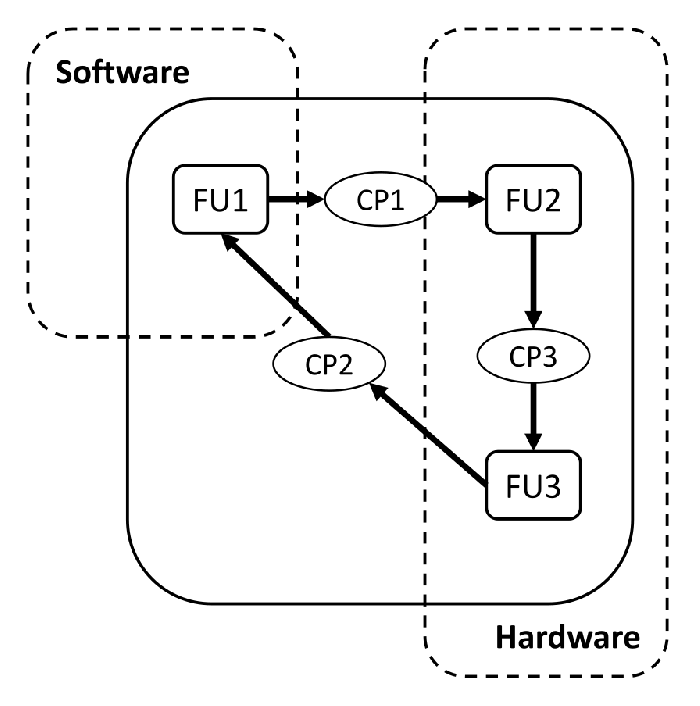
\includegraphics[width=0.49\textwidth]{example_partioning.eps}
\caption{Example of partitioning Functional Units}
\label{fig:example}
\end{figure}

\subsection{Partitioning}\label{sec:partitioning}
A designer using SystemBuilder should define a partition scheme in SDF File.
This means a designer can decide whether to implement functional units in hardware or software. For example, in \Figref{fig:example}, unit 1 is partitioned as a software process, units 2 and 3 as hardware processes.
To test another partitioning scheme, a designer has only to edit an SDF file and rerun SystemBuilder. In this way, a designer can efficiently explore a partition scheme of hardware/software. To test an implementation works as expected, a designer can run a co-simulation.
A Designer can test an implementation even faster by building all functional units as software. Since emulating software is much faster than simulating hardware, it is expected to be more efficient than running co-simulation. Co-simulation/simulation is discussed in section \ref{sec:cosimulation}.

\subsection{Functional Units (FU)}
As discussed in section \ref{sec:partitioning}, a designer can decide whether to implement a functional unit in hardware or software. However, there is a limitation. SystemBuilder uses an external high-level synthesis tool.
It means a functional unit to be implemented as a hardware process must be subjected to the external HLS tool's limitation.
On the contrary, a unit to be implemented as a software process does not have those limitations. It means that all units can be built as a software process, and it allows to test a design at a functional level.

\subsection{Communication Primitives}\label{sec:communication_primitives}
SystemBuilder supports four communication primitive as follows.

\begin{description}
  \item [Non-Blocking Communication Primitives (NBC)]\mbox{}\\
    NBC corresponds to a shared variable in software and a register in hardware.
  \item [Blocking Communication Primitives (BC)]\mbox{}\\
    BC corresponds to OS's communication feature in software and a FIFO in hardware. Access is executed by blocking in one direction.
  \item [Memory Primitives (MEM)]\mbox{}\\
    MEM corresponds to a global array in software and a dual-port memory in hardware. Access is executed by non-blocking.
    It is possible to implement a memory primitive as shared memory. In order to implement as shared memory, shared memory must be declared in an SDF file.
  \item [PreFetch BC (PFBC)]\mbox{}\\
    PFBC is a memory designed between external memory and hardware process. The purpose of PFBC is to hide latency while reading external memory. PFBC reads the bulk of data from external memory and provides fast internal memory to hardware processes connected. PFBC uses shared memory only available for the software process side; therefore, shared variables must also be declared separately.
\end{description}

These primitives can be accessed as a C language function when designing a unit.

\subsection{Synthesis} \label{sec:synthesis}
SystemBuilder takes SDF and C programs as an input and generates files for software, hardware, and interface.
% \subsubsection{Partitioning}

\subsection {Software Synthesis}
Software synthesis takes place by a compiler. It will be compiled as software running on either ITRON \cite{sakamura1987itron} or AUTOSAR-CP \cite{autosar}. Communication primitives between a software process are also implemented as software.

\subsection{Hardware Synthesis}\label{sec:hwsynthesis}
A hardware process and communication primitives between them will be synthesis as hardware. SystemBuilder uses a commercial tool to synthesis hardware processes. SystemBuilder supports the following HLS tool.

\begin{itemize}
    \item eXCite
    \item CyberWorkBech\cite{waka}
    \item Vivado HLS\cite{vivadohls}
\end{itemize}

These HLS tools support various optimization techniques such as:

\begin{itemize}
  \item Pipelining the loop to implement the operations in a loop in a concurrent manner.
  \item Unrolling the loop to exploit parallelism between loop iterations.
  \item Expanding the array signal into the individual variable.
  \item Unrolling multi-dimensional array by a dimension designer configured.
  \item Inlining the function.
\end{itemize}

In order to take advantage of these features, a designer is required to develop processes with this in mind. We had a brief compare test of pipelining the network's loop statement represented in \Tabref{tab:result} and \Tabref{tab:result2}.

\subsection{Interface Synthesis}
SystemBuilder automatically generates a hardware/software interface based on the SDF file. For the software, the device driver is generated. The device driver includes access functions, interrupt handlers, and semaphores for synchronization between hardware and software. For the hardware, the interface circuit described in HDL is generated. This interface includes glue logic that allows accessing the bus and the circuit that corresponds to communication primitives such as buffer or memory. The glue logic has an interface to a generic bus named VBUS. Therefore, SystemBuilder generates a circuit that converts protocol to connect VBUS.

\subsection{Command} \label{sec:command}
This subsection discusses the actual commands for synthesizing.

SystemBuilder provides `\texttt{SysGen}' command to synthesis the system. `\texttt{SysGen}' has the following options \cite{man:systembuilder}.

\begin{itemize}
  \item Specify the SDF file.
    \begin{description}
      \item[\texttt{-sdfy \textit{<SDF file>}}] Specify the YAML format of the SDF file.
      \item[\texttt{-sdf \;\;\textit{<SDF file>}}] Specify the sdf format of the SDF file.
    \end{description}
  \item Specify the synthesis method.
    \begin{description}
      \item[\texttt{-nobs}] Specify to not to perform high-level synthesis.
      \item[\texttt{-dobs}] Specify to perform high-level synthesis.
      \item[\texttt{-csim}] Specify to print C language level simulation.
    \end{description}
  \item Specify high-level synthesis tool.
    \begin{description}
      \item[\texttt{-bst <HLS tool name>}]
    \end{description}
  \item Specify the target board.
    \begin{description}
      \item[\texttt{-s <board name>}]
    \end{description}
  \item Specify the RTOS for running software processes.
    \begin{description}
      \item[\texttt{-os <itron or atk>}]
    \end{description}
  \end{itemize}

  `\texttt{SysGen}' commands synthesis the interface and hardware processes. It also generates `\texttt{Makefile}' for software compiles.


\subsection{Co-simulation} \label{sec:cosimulation}
To test a design, SystemBuilder supports hardware and software co-simulation. It runs RTOS emulator and RTL simulators and then coordinating them to perform co-simulation. It connects the RTOS emulator and RTL simulator by a program named device manager. The device manager runs on the host computer then connects to the RTOS emulator using an inter-process communication function from the host pc. While the RTOS emulator tries to communicate with the RTL simulator, the device manager sends a signal to the RTL simulator. The device manager uses Foreign Language Interface (FLI) to connect VBUS to the RTL simulator.

SystemBuilder supports running software processes either on QEMU or directly from the host computer. Functional Units that run on RTOS are compiled and linked with the RTOS model. Next, SystemBuilder generates an object code directly executable on the host computer \cite{honda2004rtos}. Due to native support, co-simulation speed is much faster than other simulators that simulate at the instruction-set level. In this paper, we used QEMU for the RTOS emulator and Questa Sim for the RTL simulator.

The benefit of running co-simulation is that designer can debug hardware processes. For example, a designer can observe a waveform of signals. \Figref{fig:eg_waveform} is an example of a waveform. In this figure, we can observe signals and variables.

\begin{figure}[tbp]
  \centering
  \includegraphics[width=0.99\linewidth]{questa_sim_wave.png}
  \caption{Waveform observed in Questa Sim}%
  \label{fig:eg_waveform}
\end{figure}


\subsection{Report from a HLS tool}\label{sec:report}

As a result of a high-level synthesis of hardware processes, several HDL files are created. To implement this result to the FPGA, logic synthesizing is required. At this time, the SystemBuilder requests the HLS tool to print several design reports. Design reports contain various information such as BRAM usage and LUT usage. \Tabref{tab:eg_memory} is an example of a memory usage report from Vivado. This table shows the BRAM usage of the design out of the RAM on the board. \Tabref{tab:eg_lut} is an example of LUT usage report. We can know the logic circuit size by LUT as logic usage. LUT usage can be an indicator of design efficiency.

\begin{table}[tbp]
  \centering
  \caption{Example of memory usage report}
  \label{tab:eg_memory}
  \begin{tabular}{|l|r|r|r|r|}
    \hline
Site Type         & Used & Fixed & Available & Util\% \\
\hline
Block RAM Tile       & 44.5 &     0 &       140 & 31.79  \\
\quad RAMB36/FIFO*   &   41 &     0 &       140 & 29.29  \\
\qquad RAMB36E1 only &   41 &       &           &        \\
\quad RAMB18         &    7 &     0 &       280 &  2.50  \\
\qquad RAMB18E1 only &    7 &       &           &        \\
\hline
  \end{tabular}
\end{table}

\begin{table}[tbp]
  \centering
  \caption{Example of LUT usage report}
  \label{tab:eg_lut}
  \begin{tabular}{|l|r|r|r|r|}
    \hline
                 Site Type                 &  Used & Fixed & Available & Util\% \\
\hline
Slice                                      &  3858 &     0 &     13300 & 29.01  \\
\quad  SLICEL                                   &  2587 &     0 &           &        \\
\quad  SLICEM                                   &  1271 &     0 &           &        \\
LUT as Logic                               &  9675 &     0 &     53200 & 18.19  \\
\quad  using O5 output only                     &     3 &       &           &        \\
\quad  using O6 output only                     &  7520 &       &           &        \\
\quad  using O5 and O6                          &  2152 &       &           &        \\
% LUT as Memory                              &   420 &     0 &     17400 &  2.41  \\
% \quad  LUT as Distributed RAM                   &   160 &     0 &           &        \\
% \qquad    using O5 output only                   &     0 &       &           &        \\
% \qquad    using O6 output only                   &    80 &       &           &        \\
% \qquad    using O5 and O6                        &    80 &       &           &        \\
% \quad  LUT as Shift Register                    &   260 &     0 &           &        \\
% \qquad    using O5 output only                   &     1 &       &           &        \\
% \qquad    using O6 output only                   &   231 &       &           &        \\
% \qquad    using O5 and O6                        &    28 &       &           &        \\
\hline
  \end{tabular}
\end{table}




\subsection{Workflow} \label{sec:workflow}

\begin{figure}[tb]
\centering
\includegraphics[width=0.66\textwidth]{workflowv2.eps}
\caption{Workflow inside SystemBuilder.}
\label{fig:systembuilder}
\end{figure}

In summary, we represent the workflow inside SystemBuilder in this section. \Figref{fig:systembuilder} and the following steps are an overview of workflow inside SystemBuilder.

\begin{enumerate}
    \item SystemBuilder read SDF Files and determines a partition scheme of functional units.
    \item SystemBuilder synthesis the interface between hardware and software.
    \item For software, a compiler compiles functional units with the device driver generated in step 2.
    \item For hardware, HLS Tool synthesis the code to HDL files.
    \item Users now can choose whether to run co-simulation or implement the results to FPGA.
    \begin{description}
    \item [Co-simulation] This process is described in section \ref{sec:cosimulation}.
    \item [FPGA] Logic synthesizer synthesis the HDL file created and device interface generated in step 2. This process generates design reports discussed in section \ref{sec:report}.
    \end{description}
\end{enumerate}

\section{Neural Network Console} \label{sec:nnc}

\begin{figure}[tbp]
  \centering
  \includegraphics[width=0.99\linewidth]{network_sample.png}
  \caption{Example of designing a neural network in NNC}%
  \label{fig:network_sample}
\end{figure}

A Designer can develop a network via GUI in NNC. \Figref{fig:network_sample} is an example of a network designed using NNC. As shown in this figure, NNC visualizes which layers are used in what order, from input to output.

% This section will cover the layers of NNC used in this paper. We will discuss the behavior of layers and properties. For some layers, we will also discuss the behavior at the source code level to better understand its behavior.
% the layers of NNC used in this paper. We will cover
% We will discuss the behavior of layers and properties.

This section will cover the behavior of FixedPointQuantize, convolution, affine layers of NNC. We will also discuss the behavior at the source code level to understand layers' behavior better. The source code referenced in this section is Neural Network Libraries' code, which NNC is built on.

% Neural Network Console is built on the Neural Network Libraries \cite{sony-nnabla}. This Libraries provides Python API built on the C++11 core. source code of this C+11 core.

% Neural Network Console is built on the Neural Network Libraries \cite{sony-nnabla}. This Libraries provides Python API built on the C++11 core. \Figref{fig:fixedpointquantize} is a part of source code of this C+11 core.

\subsection{FixedPointQuantize}
FixedPointQuantize layer performs linear quantization. This layer requires the following properties \cite{man:nnc}.

\begin{quote}
\begin{description}
  \item[Sign] Specify whether to include signs.
  \item[N] Specify the number of quantization bits.
  \item[Delta ($\delta$)] Specify the quantization step size.
\end{description}
\end{quote}

The FixedPointQuantize layer quantizes input and prints out data using the above properties. Printed data of the layer is not an \textbf{N}-bits integer but a float. \Figref{fig:quant_graph} is a graph that expresses the FixedPointQuantize layer's behavior. The layer's output will be the value passed through the step function. \textbf{N} is specified as four in this figure. Therefore, the number of printable data is limited to $2^\textbf{4}$. As a result, if \textbf{Sign} is true, the maximum and minimum output will be $7\delta$ and $-8\delta$. Furthermore, if \textbf{Sign} is false, the maximum and minimum output will be $15\delta$ and $0$.


\begin{figure}[tbp]
  \centering
  \begin{subfigure}[b]{0.45\textwidth}
    \centering
    \includegraphics[scale=0.35]{Quantization_graph_sign_true.pdf}
    \caption{Sign $=$ True}
    \label{subfig:quant_graph_signed}
  \end{subfigure}
  \hfill
  \begin{subfigure}[b]{0.45\textwidth}
    \centering
    \includegraphics[scale=0.35]{Quantization_graph_sign_false.pdf}
    \caption{Sign $=$ False}
    \label{subfig:quant_graph_unsigned}
  \end{subfigure}
  \caption{Graph of FixedPointQuantize layer}%
  \label{fig:quant_graph}
\end{figure}

\begin{figure}[tbp]
  \centering
  \lstinputlisting[
    language=C++,
    linerange={52-65},
    firstnumber=52
  ]{"src/fixed_point_quantize.cpp"}
  \caption{\texttt{src/nbla/function/generic/fixed\_point\_quantize.cpp}}
  \label{fig:fixedpointquantize}
\end{figure}

In order to explain the behavior more specifically, the corresponding source code is described in \Figref{fig:fixedpointquantize}. This figure is directly imported from a file. Line 54 to 57 are codes that check overflow and underflow. Line 59 to 62 are codes that check the sign of the number (\texttt{sign\_x}) and modify the value using the quantization step (\texttt{delta\_}).

By this method, it is possible to keep the FixedPointQuantize layer's output as a float. As a result, the other layers do not need to consider whether the input is quantized or not.

\subsection{Convolution}
The convolution layer convolves the input as the following equation.
\begin{equation}\label{eq:conv}
  \textbf{O}_{x,y,m} = \sum_{i,j,n} \textbf{W}_{i,j,n,m} \, \textbf{I}_{x+i,y+j,n} + \textbf{b}_m
\end{equation}
Where $\textbf{O}$ is the output, $\textbf{W}$ is the kernel weight, $\textbf{I}$ is the input, $\textbf{b}$ is the bias, $i,j$ is the kernel size, $x,y,n$ is the input index, $m$ is the output map. As the equation, it includes multiplications and additions of matrices.

\begin{figure}[tbp]
  \centering
  \lstinputlisting[
  language=C++,
  linerange={172-189},
  firstnumber=178,
  ]{"src/convolution.cpp"}
  \caption{\texttt{src/nbla/function/generic/convolution.cpp}}
  \label{fig:code_convolution}
\end{figure}


\Figref{fig:code_convolution} is the part of the convolution layer's source code.  The for loop at line 184 is where $\sum$ in the equation \ref{eq:conv} occurs. After specifying the matrix to be calculated on line 185 -- 187, the multiplication occurs on line 188. Next, the addition of bias occurs in line 191--194.


\subsection{Affine}
The affine layer is a fully-connected layer that connects all inputs to all output neurons. The following equation executes it.

\[
  o = Wi + b
\]
Where $o$ is the output, $W$ is the weight, $i$ is the input, and $b$ is the bias.

\begin{figure}[tbp]
  \centering
  \lstinputlisting[
  language=C++,
  linerange={82-90},
  firstnumber=82,
  ]{"src/affine.cpp"}
  \caption{\texttt{src/nbla/function/generic/affine.cpp}}
  \label{fig:code_affine}
\end{figure}

Similar to the convolution layer, the affine layer uses multiplication and addition of matrices. \Figref{fig:code_affine} shows the source code of the affine layer. We can observe the similarity with the convolution layer. After specifying the matrix to be calculated on line 82 -- 84, the multiplication occurs on line 85. Next, the addition of bias occurs on line 86--90.

\subsection{Max-pooling}
The max-pooling layer outputs the maximum value from the region specified by the kernel shape. This layer requires to specify the size of the kernel, stride, and padding. Stride is the number that specifies the pixels shifts over the input matrix. Padding is the number that specifies the size of zero paddings added to the ends of the input matrix before the pooling process.



\begin{figure}[tbp]
  \centering
  \lstinputlisting[
  language=C++,
  linerange={88-115},
  firstnumber=88,
  ]{"src/max_pooling.cpp"}
  \caption{\texttt{src/nbla/function/generic/max\_pooling.cpp}}
  \label{fig:code_max_pooling}
\end{figure}

\Figref{fig:code_max_pooling} shows the source code of the max-pooling layer. The variable `\texttt{y}' represents the output matrix, and `\texttt{x}' represents the input matrix.
The code in lines 91 through 96 computes the range of region to found out the maximum value. Since the input is three dimensions in the code, it finds the range of regions for each dimension.  The code in lines 97--110 finds the maximum value in the region obtained earlier.  We can see that NNC access array using multiple statements.

% !TEX root = main.tex
% !TEX encoding = UTF-8

\chapter{Model Design for SystemBuilder} \label{sec:model_design}

After generating and training a network in NNC, we convert the model for SystemBuilder to implement on FPGA. This chapter will discuss this model design for SystemBuilder using network structure and trained parameters from NNC.

\section{Overall Design} \label{sec:overall_design}

\begin{figure}[tbp]
  \centering
  \includegraphics[width=0.82\linewidth]{designed_architecture.pdf}
  \caption{Overall design of the implemented model}%
  \label{fig:designed_architecture}
\end{figure}

To use SystemBuilder, we write the System DeFinition (SDF) file that describes the overall model design. \Figref{fig:designed_architecture} is the example showing the SDF file we designed.
Communication primitives are represented as an ellipse, and functional units are represented as a rounded rectangle. The arrow leaving the unit represents the write function toward the communication primitive, and the incoming arrow represents the read function of the communication primitive. We use memory primitive to send input data to a hardware process and blocking channel primitive to send start signal and receive the inference result. If multiple hardware processes are declared as \Figref{fig:designed_architecture}, we use blocking channel primitive to communicate between hardware processes. \Figref{fig:eg_sdf} is a part of the SDF file we designed.

The input data is prepared as text and read as a global array variable in the software process, and the parameters are also prepared as text and used as global variables in each layer code.

% Software process sends start signal using BC, send image data with memory primitive, and receive inference result with BC. We designed a software process to measure the time it takes from the sending start signal to the arrival of the result. For the hardware processes, we designed it to receive the input image data and return the inference value to the software. In the case of using multiple hardware processes, we used BC as the communication primitives between hardware processes. The reason and method for using several hardware processes will be discussed in section \ref{sec:design_case_study}.



As shown in \Figref{fig:designed_architecture}, the hardware returns inferred result to SW process from the received data. For hardware process design, we take two approaches.

\paragraph{Design 1}

\begin{figure}[tbp]
  \centering
  \includegraphics[scale=0.44]{hw_process_desgin_case1.pdf}
  \caption{Single hardware process}%
  \label{fig:hw_design_1}
\end{figure}

The first approach uses a single hardware process, as shown in \Figref{fig:hw_design_1}. In this single process, several functions that play each layer's role are declared. It operates by calling each function inside the hardware process's primary function.

\paragraph{Design 2}

\begin{figure}[tbp]
  \centering
  \includegraphics[scale=0.44]{hw_process_desgin_case2.pdf}
  \caption{Multiple hardware processes}%
  \label{fig:hw_design_2}
\end{figure}

The second approach uses several hardware processes, as shown in \Figref{fig:hw_design_2}. Each process has a single function that plays the role of each layer. However, not all layer is created as a process. We create a process that corresponds to the convolution, affine, and max-pooling layers. These layers are layers that have different sizes of input data and output data. The other layers, such as an activation layer, will be built-in in the previous layer's process. For example, if one matrix element is calculated in the convolution operation, this element value passes through the activation function and is sent to the next layer.

Each process transfers one element of the resulting matrix to the next process as it is computed. The next process receives input results and then operate. Data transfer between hardware processes uses blocking channel primitive.

\section{Design of each layer}
In the previous section, we discussed the overall model design. We also discussed how the hardware processes are configured. This section will discuss the actual implemented design of three-layer, convolution, affine, and max-pooling. These layers are separately designed to be hardware process in \textbf{Design 2} of section \ref{sec:overall_design}.

We will discuss the design using the pseudocode. However, addition and multiplication in the pseudocode used are far from real. Since we are handling quantized numbers in the implementation, we take different addition and multiplication method, which will be discussed in section \ref{sec:implementation_operations}.

\subsection{Convolution}
The following code is pseudocode for the convolution layer.

\begin{quote}
\begin{lstlisting}[language=C, frame=l]
Receive results from the previous process

for (o_ch = 0; o_ch < output_channel; ++o_ch){
    for (o_h = 0; o_h < output_height; ++o_h){
        for (o_w = 0; o_w < output_width; ++o_w){

            result = 0;
            for (k_d = 0; k_d < kernel_dimension; ++k_d){
                for (k_h = 0; k_h < kernel_height; ++k_h){
                    for (k_w = 0; k_w < kernel_width; ++k_w){
                        result += input_element * kernel_element;
                    }
                }
            }
            // add bias
            result += bias_element;

            Modify result if needed (e.g. activation function)
            Print result
        }
    }
}
\end{lstlisting}


\end{quote}

The convolution layer is a layer that adds a bias to the sum of matrices multiplications. The triple for statement calculates each element of the output matrix sequentially  (line 3--5). In the inner triple loop, we access each element of the input and the kernel (line 8--10). Then, we calculate the sum of the accessed elements' multiplications (line 11) and add a bias (line 16). Next, as we discussed in section \ref{sec:overall_design}, we built some layers in one of the two hardware designs, such as an activation layer in its previous layer. In this case, it is processed (line 18). Then finally, the code print the output element (line 19).

% the if processing such as an activation function is needed, it is processed (line 18).

\subsection{Affine}
The following code is pseudocode for the affine layer.

\begin{quote}
\begin{lstlisting}[language=C, frame=l]
Receive results from the previous process

for (ch = 0; ch < output_channel; ++ch){
    result = 0;
    for (i = 0; i < input_size; ++i){
        result += input_element * parameter_element;
    }
    // add bias
    result += bias_element;

    Modify the result if needed (e.g. activation function)
    Print the result
}
\end{lstlisting}
\end{quote}

% The affine layer is a layer that adds a bias to the matrices multiplications, .

An affine layer is written in a structure similar to the convolution layer. The outer for statement calculates each output matrix element sequentially (line 3). Inner for statement calculates the sum of the multiplications (line 5--7). Like the convolution layer, after adding the bias (line 9), we modify the result if needed and print the result (line 11--12).

\subsection{Max-pooling}
The following code is pseudocode for the max-pooling layer.
\begin{quote}
\begin{lstlisting}[language=C, frame=l]
Receive results from the previous process

for (o_ch = 0; o_ch < output_channel; ++o_ch){
    for (o_h = 0; o_h < output_height; ++o_h){
        for (o_w = 0; o_w < output_width; ++o_w){

            local_max = -128;
            for (k_h = 0; h < kernel_height; ++k_h){
                for (k_w = 0; w < kernel_width; ++k_w){
                    temp = input_element;
                    if (temp > local_max) {
                        local_max = temp;
                    }
                }
            }

            Modify the local_max if needed (e.g. activation function)
            Print the local_max
        }
    }
}
\end{lstlisting}
\end{quote}

Like other designs described above, the code calculates each element of the output matrix sequentially using for statement (line 3--5). Next, it founds the largest element within the range specified by the kernel using double for statement (line 7--15). Like other designs, we modify the result and print the result (line 17--18).

% After modifying the result if needed (line 17), it print the result (line 18).



\section{Implementation of operations with quantized data}\label{sec:implementation_operations}

As discussed in section \ref{sec:nnc}, the FixedPointQuantize layer's output is a float in NNC. Therefore the other layer can be a generic usable design without considering the input is quantized or not.
% However, as we will cover in section \ref{sec:quantization}, we wanted to eliminate the use of floating-point arithmetic from our models. Therefore, we should design the layers to handle only an integer type.
However, we want to eliminate the use of floating-point arithmetic from our models. Therefore, we should design the layers to handle only an integer type.

Since we set the quantization step size ($\delta$) as the power of two, data can be expressed as follows:
% \begin{equation} % \label{eq:quant}
\[
\textrm{quantized data in original scale} = \textrm{quantized data} \times \delta, \quad \delta = 2^{-n} \; \left( n = 1, 2, \ldots\right)
\]

While `quantized data' is an integer value and $\delta$ is the quantization step.

Our model only handles this `quantized data'. Therefore, rather than the concept of passing the float data through the FixedPointQuantize layer like NNC, we designed other layers to include the concept of FixedPointQuantize layer.

Each layer receives the quantized integer as input and outputs as an integer. Quantization steps of input, output, and parameters can be different. Consequently, we take this into account when designing. This subsection will cover the implemented methods of operations with quantized data.

% , but in our model, the output of each layer is an integer with  so we have to take a slightly different approach.

\subsubsection{Addition}
Let $a$ and $b$ be defined as quantized numbers, and let $A$ and $B$ be values expressed in the original scale of $a$ and $b$. The following equations express these relations.

\begin{align*}
  A &= a \times \delta_a \\
  B &= b \times \delta_b
\end{align*}

 Since we use delta as the power of two in our implementation, let us also define $\delta_a$ and $\delta_b$ as the following equations.

\begin{align*}
  \delta_a & = 2 ^{-\alpha} \\
  \delta_b & = 2^{-\beta} \\
  \alpha,\; \beta & \in \textbf{Z}
\end{align*}

$A + B$ will be expressed as the following equation.

\begin{align*}
  A + B &= (a \times 2^{\beta - \alpha} + b) \times 2^{-\beta}
\end{align*}

Assume, without loss of generality, that $\delta_a$ is greater than or equal to $\delta_b$. Then $a \times 2^{\beta - \alpha} + b$ will be an integer. This value will be the result of the addition between quantized numbers. This value has the following meanings: The result is the addition between $a$ with adjusted quantization step and $b$. The result's quantization step will be a lower value among the operand's quantization step, which is $2^{-\beta}$ in the above equation. The following codes can express this process in the implementation.

\begin{quote}
  \lstinputlisting[language=C, numbers=left, frame=l]{"src/impl_addition.c"}
  % \caption{Implementation of addition}
  % \label{fig:addition}
\end{quote}

To decrease $a$'s quantization step by divided by $2^{\beta - \alpha}$, we increased $a$ multiplied by $2^{\beta - \alpha}$. To maximize the performance, we use a bitwise shift operation. The behavior of bitwise left shift operation with a negative number is undefined in C standard \cite{iso:c17}. Therefore, we use the if statement as line 2 to determine the negative number to solve this problem.

Variable `\texttt{a\_alter}' and `\texttt{result}' should be declared in wide-enough data type to avoid integer overflow in operation.

\subsubsection{Multiplication}

Let $a$ and $b$ use the same definition as in \textbf{Addition}. Multiplication of $a$ and $b$ can be expressed as the following equation.

\begin{align*}
  AB &= a b\times (\delta_a \times \delta_b)
\end{align*}

This equation means the result of a multiplication is $a\times b$, and the quantization step size will be the multiplication of the operand's quantization step. The following codes can express the multiplication in the implementation.

\begin{quote}
  \begin{lstlisting}[language=C, numbers=left, frame=l]
result = ((int32_t) a) * b;
  \end{lstlisting}
\end{quote}
  % \caption{Implementation of multiplication}%
  % \label{fig:multiplication}

% Multiplication can be expressed as \Figref{fig:multiplication} in the implementation.

We typecast the variable to wider data types to avoid overflow. Moreover, the variable `\texttt{result}' should be declared in a wider data type.

\subsubsection{Typecasting to narrower data types}

We store the operation result in a wider data type to implement addition and multiplication. We use a 32-bit integer to store the operation value during the process. After performing the operation required by each layer, typecasting to narrower data types is required. Each layer's output should be quantized to an 8-bit integer, not 32-bit. Moreover, we should also adjust the number's quantization step to match the output's one.



% \begin{figure}
%   \centering
%   \lstinputlisting[
%     language=C
%   ]{"src/impl_typecasting.c"}
%   \caption{Implementation of typecasting}
%   \label{fig:typecasting}
% \end{figure}

To perform this process, we use the following steps. First, we change the quantization step to match layer output. Second, we check the overflow and underflow.

% Which can be expressed as the following codes \Figref{fig:typecasting} in the implementation. In this code, we quantize variable \texttt{result} to \texttt{output}.

\paragraph{Step 1}
Changing the quantization step can be expressed as the following codes in the implementation. % In this code, we quantize variable \texttt{result} to \texttt{output}.
\begin{quote}
  \lstinputlisting[
  language=C,
  numbers=left,
  frame=l,
  linerange={1-7},
  firstnumber=1,
  ]{"src/impl_typecasting.c"}
\end{quote}

% Lines 1 to 7 are the code to change the quantization step.

In the code, it increases the quantization step by multiplied by $2^{\texttt{rescale\_amount}}$. We use the right shift operation to accomplish it. Since the right shift operation will truncate the \texttt{result}, we added a number to round it (line 2 and 5). For example, let us apply the code above to the following variable:
\begin{quote}
  \texttt{result} $=$ \texttt{0b 0100 0100}\\
  \texttt{rescale\_amount} $=$ \texttt{4}
\end{quote}
The variable `\texttt{result}' then will be ``\texttt{0b 0000 0101}''.

% Suppose we need to decrease the quantization step. In that case,
In the case of decreasing the quantization step, we can use the left shift operation method described in \textbf{Addition}. However, in the case study, the quantization step of the output always has been large or equal to the quantization step of an internal variable like `\texttt{result}'.

\subparagraph{An equivalent code in NNC}
An equivalent task happens in NNC. \Figref{fig:fixedpointquantize} is the part of the source code of the FixedPointQuantize layer. The equivalent part is line 59 -- 62 of this figure.

\begin{itemize}
  \item The concept that determines the sign of `\texttt{result}' in our model (if statement in line 1) is equivalent to lines 59, 60, and 62 of \Figref{fig:fixedpointquantize}. We design to divide the case with an if statement, but developers of NNC designs to handle with absolute values first and then handle sign next.

  \item The concept avoids truncating while left shifting is implemented in lines 2 and 5 on our models. This is equivalent to line 61 of \Figref{fig:fixedpointquantize}. The developers of NNC designs to add $0.5$ before the multiplication of quantization step (\texttt{delta\_}).
\end{itemize}


\paragraph{Step 2} Checking the overflow and underflow can be expressed as the following codes in the implementation.

\begin{quote}
  \lstinputlisting[
  language=C,
  numbers=left,
  frame=l,
  linerange={9-15},
  firstnumber=1,
  ]{"src/impl_typecasting.c"}
\end{quote}

Where \texttt{MIN} is a minimal value, and \texttt{MAX} is a maximum value of \texttt{output}'s data type. For example, if \texttt{output} is declared in an unsigned 8-bit integer, it will be \texttt{0} and \texttt{255}. Furthermore, if \texttt{output} is declared in a signed 8-bit integer, it will be \texttt{-128} and \texttt{127}.

\subparagraph{An equivalent code in NNC}
An equivalent part in NNC is line 54 -- 57 in \Figref{fig:fixedpointquantize}. However, in NNC, checking the overflow and underflow can be performed before step 1 process because the input and output are on the same scale.

% Variable \texttt{result} is 32-bit integer in our models, which can have lower quantization step compare to 8-bit integer. Therefore we did not used that method.

% !TEX root = main.tex
% !TEX encoding = UTF-8

\chapter{Case Study}
\section{Environment}
We used environment and programs as listed in \Tabref{tab:programlist}.

\begin{table}[tbp]
  \centering
  \caption{Environment and programs}
  \label{tab:programlist}
  \begin{adjustwidth}{-2in}{-2in}
  \centering
  \begin{tabular}{l|llr}\hline\hline
    Purpose & Category          & Name   & Version\\\hline
    \multirow{2}{*}{
      Running DNN framework
    }       & Host OS           & Windows 10 Pro  & 19041.746 \\
            & DNN Framework     & Neural Network Console & 1.8.7502.9306 \\\hline
    \multirow{7}{*}{
      FPGA Implemention
    }       & Host OS           & Ubuntu & 18.04.05 \\
            & System Generator  & SysGen    & 2.0 \\
            & HLS Tool          & Vivado HLS & 2019.1 \\
            & Compiler          & GCC & 6.3.1\\
            & RTL Emulator     & Questa Sim & 2019.10 \\
            & RTOS Simulator    & QEMU & 2.11.1 \\
            & Terminal Multiplexer & GNU Screen & 4.06.02 \\
            & FPGA Board        & Zybo Z7-20 & - \\\hline
    \multirow{3}{*}{
      Other Work
    }       & Host OS           & Arch Linux  & - \\
            & Image Modifier    & ImageMagick & 7.0.10.58 \\
            & CLI for nnabla    & nnabla\_cli & 1.13.0 \\\hline
  \end{tabular}
  \end{adjustwidth}
            % & CLI for  & \multirow{2}{*}{nnabla\_cli} & \multirow{2}{*}{1.13.0} \\
            % &Neural Network Libraries&&\\\hline
\end{table}
\section{DNN Models}
For the case study, we use three following DNN models provided by NNC.
\begin{itemize}
  \item Logistic regression
  \item Binary CNN
  \item LeNet
\end{itemize}

These are the network that classifies the handwriting images of Arabic numerals. Logistic regression and binary CNN classify handwriting images of 4 or 9, which binary stands for in the name of binary CNN. Unlike the previous two networks, LeNet classifies handwriting images of 0 to 9.

These three network receive an image with 28x28 pixels of one color channel as an input. We present the detail of each network in section \ref{sec:design_case_study}. Moreover, all networks we implemented can be referred to at reference \cite{webpage:nnc_project}.

% \begin{enumerate}
%   \item Implement network from running on the x86 computer. All networks were written from scratch.
%   \item Checked whether the network we created makes the same inference as NNC.
%   \item Modify the code for SystemBuilder.
%   \item Run the functional level simulation.
%   \item Confirm our network using co-simulation. We used ITRON as RTOS, and we used Vivado HLS to synthesize the hardware process.
%   \item Measure the performance on the real-machine.
% \end{enumerate}

\section{Training the network from Neural Network Console}
\subsection{Quantization} \label{sec:quantization}

Using floating-point arithmetic on FPGA would have performance degradation compared to using an integer due to higher logic requirements and speed reduction. Therefore, we did not want to use any floating-point arithmetic in our models. Since Neural Network Console supports quantization from the stage of training, we could eliminate the use of floating-point arithmetic from our models. We modified the networks to quantize the parameters and the data transfer between layers before training the network.

\begin{figure}[tbp]
  \centering
  \begin{subfigure}[b]{0.331\textwidth}
    \centering
    \includegraphics[width=\textwidth]{network_before_quant.png}
    \caption{Before}
    \label{subfig:before_quant_nnc}
  \end{subfigure}
  \quad % hfill
  \begin{subfigure}[b]{0.64\textwidth}
    \centering
    \includegraphics[width=\textwidth]{network_after_quant.png}
    \caption{After}
    \label{subfig:after_quant_nnc}
  \end{subfigure}

  \caption{Example of quantization in Neural Network Console}%
  \label{fig:quant_in_nnc}
\end{figure}

\Figref{fig:quant_in_nnc} shows the example of quantization in Neural Network Console. As the image shows, the FixedPointQuantize layer is inserted between other layers to quantize activations, and it is inserted in front of the parameter layer to quantize parameters. In this method, we were able to quantize all parameters and activations.

% \begin{equation} % \label{eq:quant}
The following equation is the equation we covered in section \ref{sec:implementation_operations}. In the case study, we quantized all parameters and activations to 8-bit integers, and we set the quantization step size ($\delta$) as the power of two.

\[
\textrm{quantized data in original scale} = \textrm{quantized data} \times \delta, \quad \delta = 2^{-n} \; \left( n = 1, 2, \ldots\right)
\]
% \end{equation}
`quantized data' is integer in the equation and $\delta$ stands for the size of 1 bit.
Since we are using $\delta$ as the power of two, we can calculate between the quantized data with low cost while implementing to FPGA. It is because we can use the shift operator for adjusting $\delta$. The detail with the operation with quantized numbers is discussed in section \ref{sec:implementation_operations}.

% However, if we use shift operations as division, it will discard the remainder. In the case of division, we add a number before shift operation to avoid this.


\subsection{Training and Accuracy} \label{sec:training_and_accuracy}
We use MNIST dataset \cite{mnist} to train and evaluate the networks. \Tabref{tab:number_mnist} shows the number of images used for training and evaluation. The accuracy measured in the evaluation are also listed in the same table.

  \begin{table}[tbp]
    \centering
    \caption{The number of images used and accuracy of the network}
    \label{tab:number_mnist}
    \begin{tabular}{l|rrrr}
      \hline\hline
      Network             & Training & Evaluation & Epoch & Accuracy \\
      \hline
      Logistic regression &  1,500   &    500     & 100   & 95.2 \% \\
      Binary CNN          &  1,500   &    500     & 100   & 98.0 \% \\
      LeNet               & 60,000   & 10,000     & 10    & 99.2 \% \\
      \hline
    \end{tabular}
  \end{table}



% \section{Implementation to FPGA}
\section{Implementation process flow}

\subsection{Preparing input data}
As we have discussed in section \ref{sec:training_and_accuracy}, we use the MNIST dataset to train and evaluate. Neural Network Console downloads and converts the MNIST dataset in PNG format to use it. We use the same PNG format of the MNIST dataset to make it easier to compare the inference results. Our main purpose is not on reading PNG images but implementing a network in FPGA. Therefore, we convert the PNG image to text for development convenience.

To prepare the image as a text, we read each pixel of an image. For the convenience of reading pixels of an image, we convert the image to BMP format. We can have the same image data because PNG and BMP are both lossless formats. We use a tool named ImageMagick \cite{imagemagick}. Following command was used.

\begin{quote}
  \begin{lstlisting}[language=bash, numbers=none, frame=l]
convert -compress none <input>.png <output>.bmp
  \end{lstlisting}
\end{quote}

The `\texttt{-compress none}' option defines not to compress the image. It is required because by default ImageMagick version 7.0.10.58 compress BMP image with a run-length encoding algorithm, making it harder to read pixels.

\begin{figure}[tbp]
  \centering
    \begin{tabular}{|p{2cm}|p{2cm}|}
    \hline
     \hfil Signature & \hfil\\
    \hline
    \multicolumn{2}{|c|}{File Size}\\
    \hline
     \hfil Reserved & \hfil Reserved\\
    \hline
    \multicolumn{2}{|c|}{File Offset to The Pixel Array}\\
    \hline
   \end{tabular}
  \caption{Bitmap File Header}
  \label{fig:bmp_header}
\end{figure}

Next, we built the program that reads each pixel of the BMP image to print it. Since the image data is not compressed, the program can open the image as binary and just read each pixel. \Figref{fig:bmp_header} shows the file header structure of BMP file. The width of the figure is 4 bytes. Therefore, the BMP format stores the offset of the pixel array at 0x0A. After reading the offset in the header, we are able to access its data.

\subsection{Preparing parameters}

After modifying the network in section \ref{sec:quantization}, and training in section \ref{sec:training_and_accuracy}, we implement it to FPGA. NNC stores the network in a binary file called `\texttt{results.nnp}'. To extract the parameter from this file, we used \texttt{nnabla\_cli} \cite{sony-nnabla}. \texttt{nnbla\_cli} is the command-line interface of Neural Network Libraries, which NNC is built on. We ran the following command to decode parameters.

\begin{quote}
  \begin{lstlisting}[language=bash, numbers=none, frame=l]
nnabla_cli decode_param -p results.nnp -o output_dir
  \end{lstlisting}
\end{quote}

This command will print out the parameters as files to `\texttt{output\_dir/}'. Data of each \texttt{Parameter} layer will be created under the directory. For example, if we decode parameters of \textbf{Figure~\ref{subfig:after_quant_nnc}}, `\texttt{Parameter.txt}' and `\texttt{Parameter\_2.txt}' will be created. \Figref{fig:parameter} is an example of decoded parameter text files. It includes the first nine lines of the parameter file. The first line indicates the matrix size of the parameter, and from the second line, the contents are recorded.

As shown in this figure, NNC stores the parameter as a float. Therefore, we quantized it to integer and stores it for use in the implementation. The parameter will be implemented as a C array in the hardware processes.

\begin{figure}[tbp]
  \centering
  \lstinputlisting[
  linerange={1-9},
  firstnumber=1,
  ]{"src/Parameter.txt"}
  \caption{Example of decoded parameter}
  \label{fig:parameter}
\end{figure}


\subsection{Designing functional units and the SDF file}

We design functional units and the SDF file as discussed in chapter \ref{sec:model_design}. After designing the functional units and SDF, we simulated the design.



% We designed a software process to send image data to FPGA, send start signals, receive results, and measure the time until receiving results. For the hardware unit, we designed it to receive the input image data and to return the inference value to the software.

% We design a System DeFinition (SDF) file for the declaration of the communication primitive between each unit. \Figref{fig:eg_sdf} is an example of the SDF file we designed for LeNet. As the figure shows, we used blocking communication primitive for communicating each hardware unit and memory primitives to commute the input image. After designing the functional units and SDF, we simulated the design.
% Due to space limitations, this figure contains only part of the file.

\subsection{Functional level simulation}
To test the design at a functional level, we simulate the design by synthesizing all units as software processes. It is useful for testing the output result of the design. If all units were synthesized as software, simulation time could be shortened since it does not go through a process such as high-level synthesis of hardware or emulating hardware using an RTL simulator.

% testing the design using co-simulation or real-machine demands more time.  However

We created a new SDF file that declares all functional units in software processes to run this simulation. We synthesize the design with the following command.

\begin{quote}
\begin{lstlisting}[language=bash, numbers=none, frame=l]
SysGen -sdfy <SDF file> -dobs -s zybo_z7_20 -bst vivado
\end{lstlisting}
\end{quote}

Each option of the command is discussed in section \ref{sec:command}. The RTOS is not specified in the command, but ITRON is used as a default for this board.

The command specifies to perform HLS. However, since there is no hardware process declared in the SDF file, HLS will not occur in this process. The command will create a new directory with the value declared as the system name (e.g. line 1 in \Figref{fig:eg_sdf}). For the functional level simulation, we use \emph{sp} as the system name. The directory `\texttt{sp/}' now has a result of synthesis. Next we change our working directory to `\texttt{\textit{sp}/fmp/}'. Then we simulate the design with the following command.

\begin{quote}
\begin{lstlisting}[language=bash, numbers=none, frame=l]
make runq
\end{lstlisting}
\end{quote}

This command compiles the software processes and runs QEMU to emulate RTOS with software processes. Next, we compare the received results with inference from NNC to determine whether the inference results were the same.

\subsection{Co-simulation}

% After testing the inference results in functional level simulation,
To debug the design, we run co-simulation. In the SDF file, the inference function must be partitioned as a hardware process in order to test the hardware behavior. To distinguish this design from the previous design in functional level simulation, we use \emph{sp\_hw} as the system's name, which indicates that the system has hardware processes.

Next, we synthesize the design with the same command discussed in functional level simulation. Unlike in the functional level simulation, we have declared the hardware processes. Therefore this command runs the HLS tool. We use Vivado for high-level synthesis.

\begin{quote}
\begin{lstlisting}[language=bash, numbers=none, frame=l]
SysGen -sdfy <SDF file> -dobs -s zybo_z7_20 -bst vivado
\end{lstlisting}
\end{quote}

 After changing the working directory to `\texttt{sp\_hw/fmp/}', we executed the following commands.

\begin{quote}
\begin{lstlisting}[language=bash, numbers=none, frame=l]
make runsim &
make runq
\end{lstlisting}
\end{quote}

The first command runs Questa Sim. Questa Sim compiles HDL files and simulates the hardware, and the second command compiles the software processes and runs QEMU to emulate the software processes. Next, we check the signal wave to debug the design. We run the following commands at Questa Sim's transcript.

\begin{quote}
\begin{lstlisting}[language=bash, numbers=none, frame=l]
add wave -position end sim:/sp_hw/*
\end{lstlisting}
\end{quote}

The wave window will now print the signal wave on its window. Then, we ran the following commands at Questa Sim's transcript to start the RTL simulation.

\begin{quote}
\begin{lstlisting}[language=bash, numbers=none, frame=l]
run -all
\end{lstlisting}
\end{quote}

Finally, after sending a start signal at QEMU, we observe the result of co-simulation.

\subsection{Implementation on the real-machine}

After co-simulation, we implement the design on the real-machine to test inference and performance. Like other processes discussed above, we synthesize the entire design and high-level synthesize the hardware with the following command.

\begin{quote}
\begin{lstlisting}[language=bash, numbers=none, frame=l]
SysGen -sdfy <SDF file> -dobs -s zybo_z7_20 -bst vivado
\end{lstlisting}
\end{quote}

Next, we run logic synthesis. SystemBuilder provides Vivado's batch script for logic synthesis. To use this, copy the files in `\texttt{Zynq/ZYBO\_Z7\_20/}' of the SystemBuilder installation path to `\texttt{sp\_hw/zynq/}' and run \texttt{run.sh}.

After logic synthesis, we connect the FPGA board to the computer and run the following command as the root account. This command implements the bitstream on the real-machine.

\begin{quote}
  \begin{lstlisting}[language=bash, numbers=none, frame=l]
make runf
  \end{lstlisting}
\end{quote}

Next, we communicate with the serial port to obtain the results. To communicate with the serial port on Linux, we did the following:

Suppose FPGA board's serial port is connected to `\texttt{/dev/ttyUSB1}'. We run the following command as the root account to display `\texttt{/dev/ttyUSB1}'.

\begin{quote}
  \begin{lstlisting}[language=bash, numbers=none, frame=l]
screen /dev/ttyUSB1 115200
  \end{lstlisting}
\end{quote}

This command connects `\texttt{/dev/ttyUSB1}' with baud rate at 115200.
Then we are able to communicate with the board via GNU Screen.


\section{Design decision of each case study} \label{sec:design_case_study}
\subsection{Logistic regression} \label{sec:logistic_regerssion}

\begin{figure}[tb]
  \center
  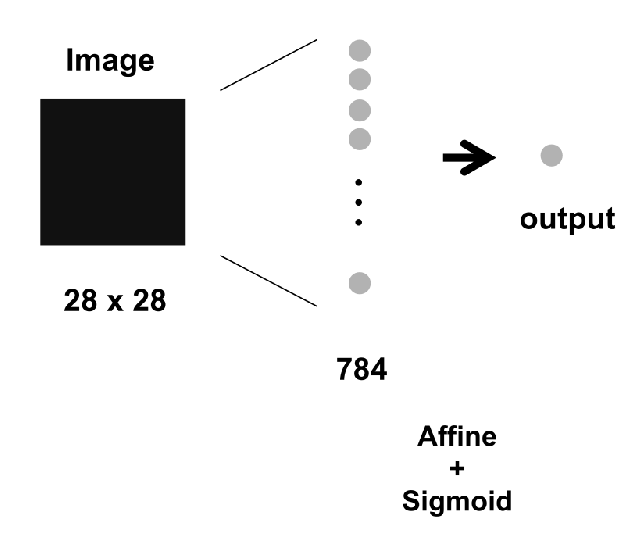
\includegraphics[width=0.41\textwidth]{affine.eps}
  \caption{Logistic regression.}
  \label{fig:affine}
\end{figure}

Logistic regression is a simple network that is formed with two layers. This network can be referred to from \Figref{fig:affine}. For hardware design, we use \textbf{Design 1} discussed in section \ref{sec:overall_design}. This hardware design is to use a single hardware process with multiple functions inside. Logistic regression is the first case study with the top priority of implementing it in an FPGA. Single hardware process design is simple comparing with multiple hardware processes design. Thus it is relatively effortless to implement the model.

To implement the activation function, we use the Taylor series of activation function that can be referenced in \cite{ccetin2015application}. However, we could not obtain the correct result by following the equation in \cite{ccetin2015application}. We expect this is because the calculations have occurred with the low precision of 8-bit integers. We made exception handling for the input that did not match the correct result to solve this problem.


\subsubsection{Pipelining the loop}

\begin{figure}[tbp]
  \centering
  \includegraphics[width=0.89\textwidth]{pipelining_loop.pdf}
  \caption{Image of pipelining the loop}%
  \label{fig:pipelining_loop}
\end{figure}

We use a loop statement to implement the matrix multiplication in an affine layer. We have tested pipelining this loop statement using HLS. \Figref{fig:pipelining_loop} depicts the concurrent execution by pipelining operations, which will shorten the computation time. Its effectiveness will be discussed in the results (section \ref{sec:results}).
% is an image of pipelining showing that implementing the operations in a concurrent manner.
% Using the HLS tool, pipelining such as the figure has applied. This will shorten the computation time. Its effectiveness will be discussed in the results (section \ref{sec:results}).

%%%%%
% After implementation, we tested the performance using pipelining and unrolling which HLS tools provided. The results refer as \ref{tab:result}.
%%%%%

\subsection{Binary CNN}\label{sec:binarycnn}

\begin{figure*}[tbp]
  \center
  \includegraphics[width=0.99\textwidth]{network_fixed.eps}
  \caption{Binary CNN}
  \label{fig:binary_cnn_network}
\end{figure*}

After successful implementation of logistic regression in section \ref{sec:logistic_regerssion}, we implement another network.
We search for the DNN Model, which includes the convolution layer. It is because we think that the convolution layer has room for further optimization with a loop statement. This room could help to test the HLS tool's optimization as future work. We use binary CNN from example networks provided by NNC \cite{webpage:nnc_project}. This network can be referred from \Figref{fig:binary_cnn_network}.

For hardware design, we use \textbf{Design 2} discussed in section \ref{sec:overall_design}. This hardware design is to use a multiple hardware process that plays each layer's role. As discussed in section \ref{sec:overall_design}, we build six hardware processes for binary CNN, corresponding to two convolution layers, two max-pooling layers, and two affine layers. Other layers are designed to be built-in to the previous layer. The reason for this design is that it will be able to test the pipelining at the layer level, which will be discussed later.

We use a lookup table for the activation layer such as Tanh and Sigmoid. As discussed in section \ref{sec:logistic_regerssion}, calculating the activation function with the low precision of 8-bit integers is challenging to achieve the correct result.

\subsubsection{Pipelining the process} \label{sec:bin_pipe}

\begin{figure}[tbp]
  \centering
  \includegraphics[width=0.4\linewidth]{pipelining_layer_buffer_size.pdf}
  \caption{Image of buffer size}%
  \label{fig:buffer_size}
\end{figure}

In the implementation of binary CNN, we use six hardware processes. Separating the hardware processes makes it possible to pipeline at the process level. We design each process to accumulate input data in a buffer until one operation is possible. When there is enough data in the buffer, it executes the operation and export the result. \Figref{fig:buffer_size} depicts this process. Suppose the outer square presents the input matrix and the inner square presents the kernel matrix.
The colored part of the figure should be accumulated in the buffer to calculate one element of the output matrix. The size of the colored part is as follows:
\[w * (w' -1) + w'\]
This will be the size of the buffer. After calculating one output element, the buffer should be shifted to store the next input element. In a case like \Figref{fig:buffer_size}, the buffer will be shifted by $w'$. After shifting, the buffer will receive a new input element. Likewise, if the buffer is full, the calculation of one output element will occur.

The method described above is slightly different from the actual implementation. The max-pooling layer is implemented in the same way as above, but the convolution layer is different. In the case of the convolution layer of binary CNN, the input matrix is three dimensions, and the kernel is also three dimensions. The concept of accumulating the buffer is the same, though there is no shifting to discard unnecessary elements. This is because unnecessary elements are not arranged in the first few elements as in two dimensions, which disallows discarding.

Using this method, we are able to pipeline the processes. We compare the pipelined and non-pipelined results.



\subsection{LeNet}
\begin{figure}[tbp]
  \centering
  \includegraphics[width=0.99\linewidth]{LeNet.pdf}
  \caption{LeNet}%
  \label{fig:lenet}
\end{figure}
For the final case study, we implement the LeNet. Unlike the other two, LeNet classifies ten kinds of input data. This network can be referred to from \Figref{fig:lenet}.

As with the design of binary CNN, we use six hardware processes to pipeline the process. We use a lookup table for the Tanh activation function. In the case of ReLu, we followed the definition of the function: if the input value is below 0, the output is 0.

\section{Results} \label{sec:results}
\subsection{Logistic regression and binary CNN}

\begin{table}[tbp]
  \caption{A result of case study including loading time of input image.}
  \label{tab:result}
  \begin{adjustwidth}{-2in}{-2in}
    \centering
    \begin{tabular}{rl|rrrr}
      \hline\hline
      Network              & Optimization     &      Latency & Throughput & BRAM Usage & LUT as Logic Util Rate\\
      \hline
      \multirow{2}{*}{
      Logistic regression} & -                &   347 $\mu$s & 2884 fps & 162 kB & 16.06 \% \\
                           & pipeline (loop) &   330 $\mu$s & 3031 fps & 162 kB & 16.61 \% \\
      \multirow{2}{*}{
      Binary CNN}          & -                & 18772 $\mu$s & 53.3 fps & 200 kB & 18.19 \% \\
                           & pipeline (process) & 18092 $\mu$s & 55.3 fps & 180 kB & 18.65 \% \\
      \hline
      \multicolumn{6}{l}{Target: ZYBO@100MHz}\\
      \multicolumn{6}{l}{Latency for Logistic regression\,: {\tt average execution time of 100-discussion}}\\
      \multicolumn{6}{l}{Latency for Binary CNN\,: {\tt average execution time of 10-discussion}}\\
    \end{tabular}
  \end{adjustwidth}
              % & & unroll   &   326 &  3066 & 160 \\
\end{table}

\begin{table}[tbp]
\caption{A result of case study without loading time of input image.}
\label{tab:result2}
  \begin{adjustwidth}{-2in}{-2in}
    \centering
    \begin{tabular}{rl|rrrr}
      \hline\hline
                   Network & Optimization & Latency & Throughput & BRAM Usage & LUT as Logic Util Rate \\
      \hline
      \multirow{2}{*}{
      Logistic regression} & -                &  61.5 $\mu$s & 16260 fps & 162 kB & 16.60 \% \\
                           & pipeline (loop) &  45.5 $\mu$s & 21978 fps & 162 kB & 16.61 \% \\
      \multirow{2}{*}{
      Binary CNN}          & -                & 18489 $\mu$s &  54.1 fps & 200 kB & 15.23 \% \\
                           & pipeline (process) & 17809 $\mu$s &  56.2 fps & 180 kB & 15.68 \% \\
      \hline
      \multicolumn{6}{l}{Target: ZYBO@100MHz}\\
      \multicolumn{6}{l}{Latency\,: {\tt execution time for 1-discussion}}\\
    \end{tabular}
  \end{adjustwidth}
                                     % & & unroll   &   326 &  3066 & 160 \\
\end{table}


For logistic regression and Binary CNN, we have confirmed that our implementation shows the same inference as the original. Next, we measure the performance of our implementation. We measure two kinds of data. One is the total latency from data transmission to output of the FPGA. This data is listed in \Tabref{tab:result}. We calculate the average of 100 inferences for logistic regression, and for Binary CNN, we use the average of 5 inferences. The other measured performance is latency without input data transmission latency, which is the network's pure computation latency. This data is listed in \Tabref{tab:result2}

The optimization column in these tables is information for comparing the applied optimization method. `pipeline (process)' means that it pipelined at the process level, and `pipeline (loop)' means that it pipelined one loop statement. This optimization method is discussed in section \ref{sec:design_case_study}.

We have tested the optimization technique in the logistic regression's implementation using the HLS tool described in section \ref{sec:hwsynthesis}. We have pipelined the loop statement in the affine layer. As a result, the throughput improved from 2884 fps to 3031 fps, resulting in a five percent performance improvement (\Tabref{tab:result}).  However, focusing on the computation time itself, throughput improved from 16260 fps to 21978 fps, resulting in a 35 percent performance improvement (\Tabref{tab:result2}).

In the implementation of Binary CNN, we experiment with pipelining in processes. As a result, throughput increased from 53.3 fps to 55.3 fps, resulting in a 3.8 percent performance improvement (\Tabref{tab:result}). Performance improvement focusing on the computation time itself was increased from 54.1 fps to 56.2 fps, resulting in a 3.9 percent performance improvement (\Tabref{tab:result2}).

\subsection{LeNet}
In the implementation of LeNet, the inference results did not match with the NNC. When we check the inference result of 10000 images, six were different from NNC.

\section{Discussion}
\subsection{The communication time}
% Comparing \Tabref{tab:result} and \Tabref{tab:result2}, it shows a laten a difference in latency of approximately 284 $\mu$s.
% This latency is the time required for the FPGA to read the image from memory.
When comparing the latencies in \Tabref{tab:result} with the latencies in \Tabref{tab:result2}, there is a consistently constant difference of about 284 $\mu$s. We believe that this consistently constant difference of latency is the time require for image data transmission to the FPGA.

The latency of binary CNN, including data transmission, is 18489 $\mu$s (without pipelining). 284 $\mu$s is about 1.0 percent of the entire latency for binary CNN. However, the entire latency of logistic regression is 374 $\mu$s (without pipelining), which leads to 284 $\mu$s to be about 82 percent of the entire latency for logistic regression. Transferring of input data is being a huge bottleneck for logistic regression. Testing other communication primitives such as prefetch BC will be worthy as future work.

\subsection{Activation function}
% Implementing a sigmoid layer or a Tanh layer from the definition might require the implementation of the exponential function. However, implementing an exponential calculation of quantized numbers was a difficult task for us.  Consequently,
We built the sigmoid function using the Taylor series in section \ref{sec:logistic_regerssion}. We suspected the loss using the Taylor series would be negligible. We thought the loss in quantizing the results would be much bigger to be able to hide the loss in the Taylor series. We used multiple Taylor series for multiple domains. We found out that the output does not monotonically increase at the boundary of each domain. We expect this is due to the low precision calculations of 8-bit integers.


To solve this problem, we took a different approach in section \ref{sec:binarycnn}. We prepared 256 ($ = 2^8$) size output an array that corresponds to 256 cases of input. We made a lookup table.

Apart from the difficulty of making, but in terms of performance and circuit size, we believe that comparing the lookup table and implementing it as a function is worthy of discussion.

\subsection{Pipelining}
\subsubsection{Observed waveform of binary CNN}
In binary CNN, we have tested the pipelining at the process level. We observed the waveform to debug its behavior.

\Figref{fig:waveform_pipeline} shows the signal between hardware processes conv1, mpool1, and conv2. These processes represent convolution, max-pooling, and convolution layer. The signal in the figure represents data transmission between processes. The signal marked as two in \Figref{fig:waveform_pipeline} represents the data transmission from mpool1 to conv2. As \Figref{fig:waveform_pipeline} shows, there is a gap between data transmission between mpool1 and conv2. This gap's latency represents the latency of accumulating the buffer of the mpool1 process. This figure shows the mpool1 process begins to calculate and print output element to next process after accumulating input element.

\Figref{fig:waveform_n_pipeline} is a waveform of binary CNN which is not pipelined. In \Figref{fig:waveform_n_pipeline}, mpool1 prints output element after receiving all input elements from conv1. This is clearly different behavior from \Figref{fig:waveform_pipeline}.

However, there is a limitation on our process level pipelined model. \Figref{fig:waveform_pipeline_overview} shows the same model as \Figref{fig:waveform_pipeline} but with larger scale. The gap marked as one is a latency before the conv2 process begins to print the result. \Figref{fig:waveform_pipeline_overview} shows conv2 begins to print result after receiving most of the mpool1's output. The convolution process of our DNN model receives three dimensions of the input matrix. Moreover, the convolution process requires matrix multiplication of a kernel matrix with the same depth as the input matrix. This leads requiring of accumulating most of the elements in the pipelining design.


\begin{figure}[tbp]
  \centering
  \includegraphics[width=0.96\linewidth]{per_pixel_detail.pdf}
    \begin{tabular}{l}
      1: Latency of accumulating the buffer at mpool1 process. \\
      2: Data transmission from mpool1 to conv2.
    \end{tabular}
  \caption{The waveform of the model pipelined at the process level}
  \label{fig:waveform_pipeline}
\end{figure}

\begin{figure}[tbp]
  \centering
  \includegraphics[width=0.99\linewidth]{per_pixel_big.pdf}
    \begin{tabular}{l}
      1: Latency of accumulating the buffer at conv2 process. \\
    \end{tabular}
  \caption{The overview waveform of the model pipelined at the process level}
  \label{fig:waveform_pipeline_overview}
\end{figure}

\begin{figure}[tbp]
  \centering
  \includegraphics[width=0.99\linewidth]{per_image_detail.png}
  \caption{The waveform of the model that did not pipeline the process}
  \label{fig:waveform_n_pipeline}
\end{figure}

\subsubsection{Efficiency}

In order to discuss the efficiency of the pipelining, we will discuss the performance gains and the increased LUT usage from pipelining. We will discuss the performance gain with the result without data transmission of an input image, represented in \Tabref{tab:result2} and discussed in section \ref{sec:results}.
% In the implementation of logistic regression, by pipelining one loop in the layer, there was about 35 percent improvement in computation speed.

\subparagraph{Logistic regression}
% In the implementation of logistic regression,
We observe about 35 percent improvement of computation speed by pipelining on loop in the process. At the same time, logic LUT usage rate increased from 16.60 \% to 16.61 \% (\Tabref{tab:result2}). The increase is about 0.1 percent. We believe that it showed high-efficiency use of logic LUT when considering the performance improvement. The amount of BRAM usage is the same as 160 kB.
% The increase in the logic LUT usage rate was 0.1 percent (\Tabref{tab:result2}).

\subparagraph{Binary CNN}
% In the implementation of binary CNN,
We observe about 3.9 percent performance improvement by pipelining at the process level. At the same time, logic LUT usage rate is increased from 15.23 \% to 15.68 \% (\Tabref{tab:result2}). The increase is about 0.45 percent. It is relatively inefficient compared to the above case, considering the degree of performance improvement.

However, BRAM usage has decreased from 200 kB to 180 kB, which can be said it is an advantage of the optimization. We suspect the BRAM has decreased because the buffer accumulating the previous layer results has decreased in each process.

\subsection{Problems of LeNet}

\begin{figure}[tbp]
  \centering
  \includegraphics[width=0.7\linewidth]{network_affine_only.png}
  \caption{Affine layer-only network}%
  \label{fig:network_affine}
\end{figure}
In the results, we found out the inference results of LeNet were different from NNC in few cases. To find out the cause, we did the following:

To find out the result of one matrix multiplication, we design a network only with one affine layer and quantization layers, as \Figref{fig:network_affine}. If we disable the affine layer's bias, the output will be the result of multiplying the input matrix and parameter matrix. This result can make us understand the matrix multiplication behavior in NNC. Matrix multiplication is also used in the convolution layer. Therefore, observing a single affine layer can help us understand the overall operation of NNC.
% This network can be referred to from \Figref{fig:network_affine}.


Next, we implement this network in the same method as the case study. When comparing the result (matrix), about half of the matrix elements showed different values. The error is at most 1; hence it is not a big error. However, we believe the accumulation of errors during the operation results in difference in the output for some cases.

The reason for the error was not known.

% !TEX root = main.tex
% !TEX encoding = UTF-8

\chapter{Conclusion}

\section{Summary}

In this paper, we review the possibility of implementing existing DNN frameworks. To achieve this, we implement three networks created and trained from NNC. In order not to use floating-point arithmetic and have the same inference result, all the data in the network was quantized from the stage of training.

For the first two case studies, we confirm that inferences from implementation were the same as those from NNC. However third case study shows the inference did not match exactly. This is an area that must be fixed through further research.

We test two approaches for finding out an efficient design. One is pipelining the matrix array (Logistic Regression), and the other is pipelining the layers (Binary CNN). As a result, we found performance gain.



\section{Future Work}
We believe that contribution of this paper will help in the future development of a tool that automatically implements the network from NNC. This tool's image is presented in \Figref{fig:autotool}. The development of this tool is our final goal.

These are some works that should be done in the future for this goal.
\begin{itemize}
  \item Find out the reason why the inference results are different in LeNet.
  \item Optimize each layer using the feature provided by HLS, such as pipelining the loop. In which explained in section \ref{sec:hwsynthesis}.
  \item Test various communication primitives described in section \ref{sec:communication_primitives}.
  \item Implement every layer that NNC supports.
  \item Build a tool that extracts network structures and create files for SystemBuilder.
  \item Explore a design of the network and make the optimal decision.
\end{itemize}

\begin{figure}[btp]
\centering
\includegraphics[width=0.58\textwidth]{automated_tool.eps}
\caption{Automated tool}
\label{fig:autotool}
\end{figure}


%%%%%%%%%%
\newpage
\bibliographystyle{unsrt}
\bibliography{bib.bib}

%%%%%%%%%%
\newpage
% !TEX root = main.tex
% !TEX encoding = UTF-8

\subsubsection*{Acknowledgment}

I want to express my deep gratitude to Professor Edahiro and Professor Honda, for their guidance and critiques of this research work. I would also like to thank to Dr. Yamamoto for his useful advice and assistance in keeping my progress on schedule. I would also like to extend my thanks to the people at the Edahiro laboratory to offer me the resources in running the program.

% \clearpage

%%%%%%%%%%
% !TEX root = main.tex
% !TEX encoding = UTF-8

\pagenumbering{gobble}
\thispagestyle{empty}
% \oddsidemargin -2.5in
% \evensidemargin -2.5in
\topmargin -.5in
% \marginparwidth = 0pt

% \begin{adjustwidth}{-1.25in}{-1.25in}
% \end{adjustwidth}
\begin{flushright}
  \begin{turn}{-90}
    % \small
    Efficient Hardware Design of Quantized DNN Inference Using HLS and DNN Framework
    \qquad
    \qquad
    \quad
    \quad
    % \textbf{February, 2021}
    {\ja 2021年2月}
    \qquad
    \qquad
    \quad
    \quad
    KIM Hyunjae
%     \begin{minipage}{8.0in}
%      \small
%      %\footnotesize
%      \hfill
%      \textbf{2020-02}
%      \hfill
%      \textbf{KIM Hyunjae}
%    \end{minipage}

  \end{turn}

\end{flushright}

\end{document}
